\documentclass[10pt,a4paper]{article}
\usepackage[utf8]{inputenc}
\usepackage[english]{babel}
\usepackage{amsmath}
\usepackage{amsfonts}
\usepackage{amssymb}
\usepackage{makeidx}
\usepackage{graphicx}
\usepackage{lmodern}
\usepackage{bm}
\usepackage[numbers]{natbib}
\usepackage{tikz}
\usepackage{amsthm}
\usetikzlibrary{calc}
\usepackage[left=2cm,right=2cm,top=2cm,bottom=2cm]{geometry}
\usepackage{thmtools, thm-restate}

\author{Djordje Zivanovic}
\title{\textbf{Warsaw PhD Open Course: From Joins to Aggregates and
Optimization Problems - Exam solutions}}
\begin{document}
\maketitle
\bigskip
%Chapter 1 in Ockendon \& Tayler: Applied PDE's  
%{\it Maths Institute Lecture Notes}. 	
%{\bf Exercises 1, 2, 4, 5}.
\newcommand{\transpose}[1]{#1 ^ \text{T}}
\newcommand{\mat}[1]{\textbf{\text{{#1}}}}
\newcommand{\vect}[1]{\mat{#1}}
\newcommand{\gradient}[1]{\nabla_{\vect{#1}}}
\newcommand{\der}[1]{\frac{\partial}{\partial #1}}
\newcommand{\numberthis}{\addtocounter{equation}{1}\tag{\theequation}}
\newcommand{\logfun}{\sigma(\transpose{\vect{x}}_i \vect{w})}
\newcommand{\softmaxi}{\frac{e^{z_i}}{\sum_{l=1}^Ce^{z_l}}}
\newcommand{\layersep}{2.5cm}
\newcommand{\layersepH}{6cm}
\newcommand{\layersepP}{7cm}
\newcommand{\layersepB}{9cm}
\newtheorem{theorem}{Theorem}
\newtheorem{lemma}[theorem]{Lemma}

\newtheorem{conjecture}[theorem]{Conjecture}
\begin{enumerate}
\item[1]
Let $Q(\mathbf{A_1} \cup \mathbf{A_2} \cup \cdots \cup \mathbf{A_n})$ denote a join query on relations $R_1(\mathbf{A_1})=R_1(A_1, A_2), \cdots R_n(\mathbf{A_n})=R_n(A_n, A_1)$.

Let $\mathcal{H}=(\mathcal{V}, \mathcal{E})$ denote a corresponding hypegraph to the join query, then $\mathcal{V} = \{A_1, .., A_n\}$ and $\mathcal{E} =\{\{A_1, A_2\}, ..., \{A_n, A_1\}\}$.
\begin{enumerate}
\item[1.1]
Let $x_{R_i}$ denote the weight of an hyperedge (relation) $R_i$ in the join query $Q$. In addition let $cover_i$ denote the set of relations corresponding to edges that are part of the cover for the variable $i$. The fractional edge cover number $\rho^{*}(Q)$ is the cost of an optimal solution to the linear program:
\begin{eqnarray}
\text{minimize} \sum_{i\in [n]} x_{R_i}  \label{eq:minimize} \\
\text{subject to} \sum_{rel_j \in cover_i} x_{rel_j} \geq 1, i \in [n]  \label{eq:inequalities}\\
x_{R_i} \geq 0, i \in [n] \nonumber
\end{eqnarray}

By a definition of a cover, only edges incident  to variable are part of its cover. Thus, in our case $cover_i =\{ R_{i-1}, R_i \}$, where $R_0$ is $R_n$ in the case of $A_1$. If we rewrite the inequalities \ref{eq:inequalities} we will get:
\begin{eqnarray}
x_{R_1} +  x_{R_n} \geq 1 \nonumber \\
x_{R_1} +  x_{R_2} \geq 1\nonumber \\
\vdots \nonumber \\
x_{R_{n-1}} +  x_{R_n} \geq 1 \nonumber
\end{eqnarray}
By summing inequalities we get:
$$2\left(\sum_{i\in [n]} x_{R_i}\right) \geq n$$
\end{enumerate}
This means the minimized function $\rho^*(Q)$ cannot  be less than $\frac{n}{2}$. This is achievable if we set $x_{R_i}=\frac{1}{2}, i \in [n]$. We can see that this solution satisfies all constraints in the linear program. Finally, $\rho^*(Q)=\frac{n}{2}$. 
\\
A width of a specific hypertree decomposition is defined as a maximum among all edge covers for each of the nodes of the hypertree. A hypertree width (htw) for the specific query Q is defined as a minimum width among all possible widths of hypertree decompositions of a query Q. 
\\
A fractional width of a specific hypertree decomposition is defined as a maximum among all fractional edge covers for each of the nodes of the hypertree. A fractional hypertree width (fhtw) for the specific query Q is defined as a minimum width among all possible widths of hypertree decompositions of a query Q.
The only difference is that in the case of fractional hypertree width we use fractional edge covers instead of edge covers. \\
In the case of $n=2$ $fhtw(Q) = htw(Q) = 1$. For $n >= 3$ the hypertree decomposition on the figure \ref{fig:fthw} is the optimal one. From picture we can figure out that $htw(Q)=2$ in all cases, while $fhtw(Q)=2$ for $n>3$, but for $n=3$ it is $\frac{3}{2}$. 
\\
The decomposition on the figure \ref{fig:fthw} is optimal because we have to "propagate" one variable through nodes of the hypertree in order to fulfill the condition that all hyperedges of hypergraph are contained in the nodes of hypertree. Adding more than three variables inside a node of hypertree would increase (fractional) width of a hypertree decomoposition because we would need to cover at least two variables that are not in the same relation.  (Fractional) edge cover number for each of nodes of hypegraph inside nodes of hyperetree is $2$ because $A_1 A_iA_{i-1}$ can be covered with $x_{R_i}=1, x_{R_1}=1$. The only exception to the previous case is $n=3$ where fractional edge cover of $\frac{3}{2}$ is possible. 
\begin{figure}
\begin{center}
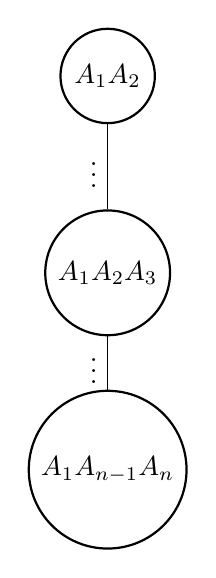
\begin{tikzpicture}
\begin{scope}[every node/.style={circle,thick,draw}]
    \node (C) at (2.5,2.5) {$A_1 A_2$};
    \node (D) at (2.5,0) {$A_1 A_2 A_3$};
    \node (E) at (2.5,-2.5) {$A_1 A_{n-1}A_{n}$};
\end{scope}
\begin{scope}
    \path  (C) edge node {$\vdots$    \, \,} (D);
    \path[]  (D) edge node {$\vdots$    \, \,} (E);
\end{scope}
\end{tikzpicture} 
\end{center}
\caption{Hypertree decomposition that corresponds to fhtw}
\label{fig:fthw}
\end{figure}

\item[1.2]
A size of listing representation is $\mathcal{O}(N^{\rho^*(Q)})=\mathcal{O}(N^{\frac{n}{2}})$ and can be computed in time $\mathcal{O}(N^{\rho^*(Q)})=\mathcal{O}(N^{\frac{n}{2}})$. Let $|D|$ represent a size the of training data set which is the number of tuples in the join of all relations $R_1, R_2, ..., R_n$. Let $\mat{X}$ represent training data set consisting of tuples of the join with an additional intercept column with values only 1. Let $\vect{y}$ represent labels of training data corresponding to tuples of join and let $\theta$ be a column vector of training parameters for all features and a bias. In addition, let $\lambda$ represent hyperparemeter of $\ell_2$ regularizer.
A loss function with added $\ell_2$ regularizer is :
\begin{eqnarray}
2|D|\mathcal{L}(\mat{X},\vect{y}, \mathbf{\theta})  &=& (\vect{y} - \mat{X}\mathbf{\theta})^2 \nonumber + \lambda |D| ||\mathbf{\theta}||_2^2\\
			&=& \transpose{(\vect{y} - \mat{X}\mathbf{\theta})}(\vect{y} - \mat{X}\mathbf{\theta}) + \lambda |D| ||\mathbf{\theta}||_2^2 \nonumber \\
&=&\transpose{\vect{y}}\vect{y} - \transpose{\vect{y}}\mat{X}\mathbf{\theta}
- \transpose{\mathbf{\theta}}\transpose{\mat{X}} \vect{y}
+ \transpose{\mathbf{\theta}}\transpose{\mat{X}}\mat{X}\mathbf{\theta} + \lambda |D| |\mathbf{\theta}||_2^2 \nonumber \\
&=&
\transpose{\vect{y}}\vect{y} - 2 \transpose{\vect{y}}\mat{X}\mathbf{\theta}
+ \transpose{\mathbf{\theta}}\transpose{\mat{X}}\mat{X}\mathbf{\theta} + \lambda |D| \transpose{\mathbf{\theta}}\mathbf{\theta}
\label{eq:loss}
\end{eqnarray}
In the equation \ref{eq:loss} we used the property that transpose of a scalar is the same scalar. All equations before that are simple vector multiplications and additions. 
Finally: 
$$\mathcal{L}(\mat{X},\vect{y}, \mathbf{\theta}) = 
\frac{1}{2|D|} \transpose{\vect{y}}\vect{y} - \frac{1}{|D|} \transpose{\vect{y}}\mat{X}\mathbf{\theta}
+ \frac{1}{2|D|}\transpose{\mathbf{\theta}}\transpose{\mat{X}}\mat{X}\mathbf{\theta} + 
\frac{\lambda}{2} \transpose{\mathbf{\theta}}\mathbf{\theta}
$$
If we derive the equation \ref{eq:loss} we get the gradient of the loss function for one point:
\begin{eqnarray}
\nabla_{\mathbf{\theta}} \mathcal{L}(\mat{X},\vect{y}, \mathbf{\theta}) &=& 0  - \frac{1}{|D|}\transpose{\mat{X}}\vect{y} + \frac{1}{|D|}\transpose{\mat{X}}\mat{X}\mathbf{\theta} + \lambda \mathbf{\theta} \nonumber \\
&=& \frac{1}{|D|}\transpose{\mat{X}}\mat{X}\mathbf{\theta} - \frac{1}{|D|}\transpose{\mat{X}}\vect{y} + \lambda \mathbf{\theta}\nonumber
\end{eqnarray}
Here we used properties $\gradient{\vect{x}}(\transpose{\vect{x}}\mat{A}\vect{x})=\mat{A}\vect{x} + \transpose{\mat{A}}\vect{x}$, $\gradient{\vect{x}}(\transpose{\vect{x}}\vect{x})=2\vect{x}$, $\gradient{\vect{x}}(\transpose{\vect{c}} \vect{x}) = \vect{c}$. In addition we used $\transpose{\left(\vect{u} \vect{v}\right)} = \transpose{\vect{v}}\transpose{\vect{u}}$. \\
A gradient descent formula is:
$$\mathbf{\theta}_{t+1}=\mathbf{\theta}_t - \eta\nabla_{\mathbf{\theta}} \mathcal{L}(\mat{X},\vect{y}, \mathbf{\theta})$$
where $\theta_t$ represents parameters in the $t$-th iteration (we start with $\theta_0$ ) and $\eta$ represents hyperparameter of gradient learning.  
\\
After joining relations we need in each step to calculate gradient. 
We can notice that $\transpose{\mat{X}}\vect{y}$ can be cached and the complexity to do so is $\mathcal{O}(n \cdot N^\frac{n}{2})$. Similarly with $\transpose{\mat{X}}\mat{X}$, whose calculation takes $\mathcal{O}(n^2 \cdot N^\frac{n}{2})$. In each iteration we need to multiply $\transpose{\mat{X}}\mat{X}$ with $\mathbf{\theta}$ which takes $\mathcal{O}(n^2)$ time. We will ignore additions of vectors because they are one $O(n)$.   
When we add  all time complexities we get:
$$\mathcal{O}(N^\frac{n}{2} + n^2 \cdot N^\frac{n}{2} + n \cdot  N^\frac{n}{2} + n^2 \cdot t) $$
If we refined the complexity and included the fact that categorical variables behave as the vectors whose length is the same as a length of the particular domain, the complexity would become:
$$\mathcal{O}(N^\frac{n}{2} + (n_d)^2 \cdot N^\frac{n}{2} + n_d \cdot  N^\frac{n}{2} + n_d^2 \cdot t) $$
where $n_d= n - 3 +  |Dom_{A_1}|+|Dom_{A_2}| + |Dom_{A_3}|$.
Memory complexity after the join is
$\mathcal{O}(N^\frac{n}{2})$. $\transpose{\mat{X}}\mat{X}$ cached takes $\mathcal{O}(n^2)$ and $\transpose{\mat{X}}\vect{y}$ takes $\mathcal{O}(n)$.
When we add these complexities we get memory complexity at each iteration is:
$\mathcal{O}(n^2)$. In addition, if we include in the result the fact that we have categorical values, memory complexity is $\mathcal{O}(n_d^2)$. 

\item[1.3]
If we denote $\mathbf{\Sigma} = \frac{1}{|D|}\transpose{\mat{X}} \mat{X}, \vect{c} = \frac{1}{|D|}\transpose{\mat{X}}\vect{y}, $
and elements of these tensors, respectively, $\mathbf{\sigma}_{ij}, \vect{c}_{i}$ then FAQs for $\Sigma$ are: 
\begin{itemize}
\item When i-th feature and j-th feature are continuous values. 
$$|D| \cdot \mathbf{\sigma}_{ij}= \sum_{a_1 \in Dom(A_1)} \sum_{a_2 \in Dom(A_2)} \cdots \sum_{a_n \in Dom(A_n)} a_i \cdot a_j 
\prod_{k\in[n]} \vect{1}_{R_k(a_k, a_{k+1})}$$
\item When i-th feature is a categorical value and j-th feature is a continuous value. 
$$|D| \cdot \mathbf{\sigma}_{ij}[a_i]= \sum_{a_1 \in Dom(A_1)} \sum_{a_2 \in Dom(A_2)} \cdots 
\sum_{a_{i-1} \in Dom(A_{i-1})}
\sum_{a_{i+1} \in Dom(A_{1+1})}
\cdots
\sum_{a_n \in Dom(A_n)}  a_j 
\prod_{k\in[n]} \vect{1}_{R_k(a_k, a_{k+1})}$$
\item When i-th feature and j-th feature are categorical values. 
$$|D| \cdot \mathbf{\sigma}_{ij}[a_i, a_j]= 
\sum_{\substack{a_{1} \in \\Dom(A_{1})}}
\sum_{\substack{a_{2} \in \\Dom(A_{2})}}
\cdots 
\sum_{\substack{a_{i-1} \in \\Dom(A_{i-1})}}
\sum_{\substack{a_{i+1} \in \\Dom(A_{i+1})}}
\cdots
\sum_{\substack{a_{j-1} \in \\Dom(A_{j-1})}}
\sum_{\substack{a_{j+1} \in \\Dom(A_{j+1})}}
\cdots
\sum_{a_n \in Dom(A_n)}  
\prod_{k\in[n]} \vect{1}_{R_k(a_k, a_{k+1})}$$

\end{itemize}
If we calculate $\sigma_{ij}$ we don't need to calculate $\sigma_{ji}$ because $\Sigma$ matrix is symmetric, therefore $\sigma_{ij} =\transpose{\sigma_{ij}}$ \\
For $\vect{c}$ FAQs:
\begin{itemize}
\item When i-th feature and label are  continuous values: 
$$|D| \cdot \mathbf{c}_{i}= \sum_{a_1 \in Dom(A_1)} \sum_{a_2 \in Dom(A_2)} \cdots \sum_{a_n \in Dom(A_n)} a_i \cdot a_n 
\prod_{k\in[n]} \vect{1}_{R_k(a_k, a_{k+1})}$$
\item When i-th feature is a categorical value and label is a continuous value: 
$$|D| \cdot \mathbf{c}_{i}[a_i]= \sum_{a_1 \in Dom(A_1)} \sum_{a_2 \in Dom(A_2)} \cdots 
\sum_{a_{i-1} \in Dom(A_{i-1})}
\sum_{a_{i+1} \in Dom(A_{1+1})}
\cdots
\sum_{a_n \in Dom(A_n)}  a_n 
\prod_{k\in[n]} \vect{1}_{R_k(a_k, a_{k+1})}$$
\item When i-th feature and label are categorical values: 
$$|D| \cdot \mathbf{c}_{i}[a_i, a_n]= 
\sum_{\substack{a_{1} \in \\Dom(A_{1})}}
\sum_{\substack{a_{2} \in \\Dom(A_{2})}}
\cdots 
\sum_{\substack{a_{i-1} \in \\Dom(A_{i-1})}}
\sum_{\substack{a_{i+1} \in \\Dom(A_{i+1})}}
\cdots
\sum_{a_{n-1} \in Dom(A_{n-1})}  
\prod_{k\in[n]} \vect{1}_{R_k(a_k, a_{k+1})}$$
\end{itemize}
Just let us notice that $a_{n+1}=a_1$ for notational purposes, $i \in [n-1] \cup \{0\} $, where $0$ represents intercept column feature. In cases where one of the features is intercept feature, there is no "skip" in sums over the intercept feature.
Here we used $\mathbf{1}_E$ which is the Kronecker delta that evaulates to 1(0) whenever the event $E$ (not) holds. $R_k(a_k, a_{k+1})$ evaluates to 1(0) whenever tuple $(a_k, a_{k+1})$ is a part of relation $R_k$. 
If we wanted FAQs per definition from the slides we would:
\begin{itemize}
\item set $\psi_k=\vect{1}_{R_k(a_k, a_{k+1})}$, except in the case of $\psi_{i}$ and $\psi_j$ where the expression above is multiplied by $a_i$, $a_j$.
\item set $\oplus = \sum$
\item set $\otimes = \prod$
\item set free variables to corresponding categorical variables if there are any. For instance, in the case when there is one categorical variable a free variable would be that variable. 
\end{itemize}
According to the \cite[page 7]{abo2018database}  complexity 
$$
\mathcal{O}\left(|\mathcal{V}|^{2} \cdot|\mathcal{E}| \cdot \sum_{i, j \in[n-1]\cup\{0\}}\left(N^{\mathrm{faqw}(i, j)}+\left|\sigma_{i j}\right|\right) \cdot \log N\right)
 $$
 where $ \mathrm{faqw} \leq \mathrm{fhtw} + c - 1$ where $c$ is maximum of categorical variables for any $\sigma_{ij}$. In the case when we have only continuous variables $\mathrm{faqw} =\mathrm{fhtw}$ the previous complexity is then 
 $$
\mathcal{O}\left(|\mathcal{V}|^{2} \cdot|\mathcal{E}| \cdot \sum_{i, j \in \{4, 5, ..., n-1\}\cup\{0\}}N^{\mathrm{2}}\cdot \log N\right) = \mathcal{O}\left(n^5 N^{\mathrm{2}}\cdot \log N\right)
 $$
 For categorical case we would join relations one by one leaving categorical variables (relations to whom they belong) the last with each join taking the most $O(N^2)$ and keeping aggregates (in this case count).  By doing this we can get final join in $O(n \cdot N^2 \cdot \log N)$ (which is what the slides claim).\footnote{Further explanations omitted due time constraints}
\item [1.4]
By properties of functional dependency $A_2 \rightarrow A_1A_3 \Leftrightarrow A_2 \rightarrow A_1, A_2\rightarrow A_3$. This means if we one-hot encode each of categories from variables $A_1, A_2, A_3$ then $\vect{a}_{A_1} = \mat{R}_1 \vect{a}_{A_2}$ and $\vect{a}_{A_3} = \mat{R}_3 \vect{a}_{A_2}$ due to functional dependencies. Furthermore, if we concatenate particular matrices $\mat{R}= \begin{bmatrix}
\mat{R}_1 \\
\mat{R}_2
\end{bmatrix}
$  
and 
$\vect{a}_{A_1A_3}= \begin{bmatrix}
\vect{a}_{A_1} \\
\vect{a}_{A_3}
\end{bmatrix}
$, we get $\vect{a}_{A_1A_3}=\mat{R}\vect{a}_{A_2}$. Approximation of output based on $\theta s$ is:
\begin{eqnarray}
\hat{y} &=& 
\sum_{ i\in [n-1] \setminus \{ 1, 2,3 \} \cup \{0\}} \langle \theta_i, \vect{x}_i \rangle + \langle \theta_1 , \vect{x}_1 \rangle  + \langle \theta_2 , \vect{x}_2 \rangle + \langle \theta_3, \vect{x}_3 \rangle\\
&=&
\sum_{ i\in [n-1] \setminus \{ 1, 2,3 \} \cup \{0\}} \langle \theta_i, \vect{x}_i \rangle + \langle \theta_{13},\vect{x}_{13} \rangle  + \langle \theta_2, \vect{x}_2 \rangle \rangle\\
&=&
\sum_{ i\in [n-1] \setminus \{ 1, 2,3 \}\cup \{0\}} \langle \theta_i, \vect{x}_i \rangle + \langle \theta_{13},\mat{R} \vect{x}_2 \rangle  + \langle \theta_2 ,\vect{x}_2 \rangle \rangle\\
&=&
\sum_{ i\in [n-1]\setminus \{ 1, 2,3 \} \cup \{0\}} \langle \theta_i, \vect{x}_i \rangle +   \langle \transpose{\mat{R}} \theta_{13} +\theta_2 ,\vect{x}_2 \rangle \rangle \label{eq:approximation}\\
\end{eqnarray}
Let $\gamma_2 = \transpose{\mat{R}}\theta_{13} + \theta_2$ and let $\gamma_j = \theta_j, j \in \{0, 4, ..., n-1\}$. Then $\gamma_j$ won't appear in the loss function because they don't appear in $\hat{y}$ as we see in the equation \ref{eq:approximation}. They still appear in l2 regularizer. In the l2 regularizer we have:
$$\frac{\lambda}{2} \sum_{j \in \{0, 4, 5, ..., n \} } ||\gamma_j||_2^2 + ||\theta_{13} ||^2_2 +  ||\gamma_2 - \transpose{\mat{R}}\theta_{13}  ||$$
By optimizing out (we reach optimal value) $\theta_{13}$ from regularizer we get 
$$\frac{1}{\lambda} \frac{\partial l2}{\partial \theta_{13}} =\mat{R}(\transpose{\mat{R}}\theta_{13} - \gamma_2) + \theta_{13} =0$$
which by further solving we get:
$$\theta_{13} = (\mat{I} + \mat{R}\transpose{\mat{R}})^{-1}\mat{R}\gamma_2$$
Finally l2 regularizer is:
$$\frac{\lambda}{2} \sum_{j \in \{0, 4, 5, ..., n-1 \} } ||\gamma_j||_2^2 + \langle (\mat{I} + \transpose{\mat{R}}\mat{R})^{-1}, \gamma_2 \rangle $$ (the full derivation in the "Learning Models over Relational Data
using Sparse Tensors and Functional Dependencies").
If we refined the complexity and included the fact that categorical variables behave as the vectors whose length is the same as a length of the particular domain, the complexity would become:
$$\mathcal{O}(N^\frac{n}{2} + (n_d)^2 \cdot N^\frac{n}{2} + n_d \cdot  N^\frac{n}{2} + n_d^2 \cdot t) $$
where $n_d= n + |Dom_{A_1}|+|Dom_{A_2}| + |Dom_{A_3}|$.
We have reduced unnecessary operations from three categorical variables to one, which reduces $n_d$ to $n_w = n + |Dom_{A_2}|$
$$\mathcal{O}(N^\frac{n}{2} + (n_w)^2 \cdot N^\frac{n}{2} + n_w \cdot  N^\frac{n}{2} + n_w^2 \cdot t) $$
\item[2.]
\item[2.1]

The OuMv problem is:
\begin{itemize}
\item 
Input an $n \times n$ Boolean matrix \mat{M} and $n$ pairs $(\vect{u}_1, \vect{v}_1), ..., (\vect{u}_n, \vect{v}_n)$ of Boolean column-vectors of size $n$ arriving one after the other. 
\item 
	Goal is after seeing each pair $(\vect{u}_r, \vect{v}_r)$ to output $\transpose{\vect{u}_r}\mat{M}\vect{v}_r$.
\end{itemize}
\begin{conjecture}\label{conj:OUVM}
For any $\gamma > 0$, there is no algorithm that solves the OuMv problem in time $\mathcal{O}(n^{3-\gamma})$.
\end{conjecture}
Let us assume there is an algorithm $\mathcal{A}$ which maintains 4-cycle detection with update time $\mathcal{O}(N^{\frac{1}{2}-\gamma})$, pre-processing time $\mathcal{O}(N^2)$, and answer time $\mathcal{O}(1)$ over a database of size $N$, unless the OuMv conjecture fails. 
The algorithm  $\mathcal{B}$ using algorithm $\mathcal{A}$ which solves OuMv in subcubic time is:
\begin{itemize}
\item[(1)] 
Insert at most $n^2$ tuples in $R$ such that $R(A, B) = \{(i, j) | \mat{M}(i, j) = 1\}$ and in $T$ such that $T(C, D) = \{(j, i) | \mat{M}(i, j) = 1\}$ ;
\item[(2)] In each round $r \in [n]$:
\begin{itemize}
\item[(2.1)] Delete all tuples in in $S, W$;
\item[(2.2)]  Insert at most $2n$ tuples into $S,  W$ 
$S(B, C) = \{(j, j) | \vect{v}_r(j) = 1\}$
$W(D, A) = \{(i, i) | \vect{u}_r(i) = 1\}$;
\item[(2.3)] Check $R \bowtie S \bowtie T \bowtie W \neq \emptyset$. This holds only iff $\transpose{\vect{u}}_r\mat{M}\vect{v}_r=1$
$
\exists i, j \in[n] \text { with } \vect{u}_{r}(i)=1, \mat{M}(i, j)=1, \text { and } \vect{v}_{r}(j)=1
$.
Time analysis:
\end{itemize}
\end{itemize}
There are at most $n^2$ tuples inserted at the step (1) and $2n$ at the step 2, thus the size of database is at most $O(n^2)$, because tuples from the step $2$ are deleted in each round. 
A complexity of the step (1) of algorithm $\mathcal{B}$ is:
$$\mathcal{O}(n^2 \cdot (n^2)^{\frac{1}{2} -\gamma}) =
\mathcal{O}(n^2 \cdot n^{1- 2 \gamma }) = \mathcal{O}(n^{3-2\gamma})$$
Here we calculated complexity of inserting $n^2$  tuples to the database.  
A complexity of the step (2) of algorithm $\mathcal{B}$ is:
$$\mathcal{O}(4n \cdot (n^2)^{\frac{1}{2} -\gamma} + 1) = \mathcal{O}(4 n^{2-2\gamma} + 1 ) = \mathcal{O}(n^{2-2\gamma})$$
The analysis of the step (2) takes into consideration that there are at most $2n$  tuples to be deleted and inserted from $S, W$ ($\vect{u}_r$ and $\vect{v}_r$ are filled with ones).
Time for $n$ rounds in the step (2) is:
$$\mathcal{O}(n \cdot n^{2-2\gamma})=\mathcal{O}(n^{3-2\gamma})$$ 
Summing complexities of steps (1) and 2) we get that an overall time complexity is $\mathcal{O}(n^{3-2\gamma})$, which is in contradiction to the claim from the conjecture \ref{conj:OUVM}. 

\item[2.2]

\end{enumerate}


\bibliographystyle{IEEEtranN}
\bibliography{research}

\end{document}